%http://www.maths.manchester.ac.uk/~kd/latextut/pdfbyex.htm
\documentclass[a4paper,twoside]{article}      % Comments after  % are ignored
\usepackage{amsmath,amssymb,amsfonts} % Typical maths resource packages
\usepackage{graphics}                 % Packages to allow inclusion of graphics
\usepackage{graphicx}
\usepackage{color}                    % For creating coloured text and background
\usepackage{hyperref}                 % For creating hyperlinks in cross references
\usepackage{listings}

\usepackage{color}
\usepackage{listings}
%\usepackage{textcomp}
\usepackage{setspace}
%\usepackage{palatino}

\newenvironment{codelisting0}
{\begin{list}{}{\setlength{\leftmargin}{1em}}\item\tiny}
{\end{list}}

\renewcommand{\lstlistlistingname}{Code Listings}
\renewcommand{\lstlistingname}{Code Listing}
\definecolor{orange}{rgb}{1,0.5,0}
\definecolor{gray}{gray}{0.5}
\definecolor{green}{rgb}{0,0.5,0}
\definecolor{lightgreen}{rgb}{0,0.7,0}
\definecolor{purple}{rgb}{0.5,0,0.5}
\definecolor{darkred}{rgb}{0.5,0,0}

%%% ----- commented out -------- Philipp --- 2010-11-09 ----------
%%%\lstnewenvironment{code}[1][]{
%%%\lstset{ %
%%%language=XML,                % choose the language of the code
%%%basicstyle=\footnotesize,       % the size of the fonts that are used for the code
%%%numbers=left,                   % where to put the line-numbers
%%%numberstyle=\footnotesize,      % the size of the fonts that are used for the line-numbers
%%%stepnumber=1,                   % the step between two line-numbers. If it's 1 each line will be numbered
%%%numbersep=5pt,                  % how far the line-numbers are from the code
%%%backgroundcolor=\color{black},  % choose the background color. You must add \usepackage{color}
%%%showspaces=false,               % show spaces adding particular underscores
%%%showstringspaces=false,         % underline spaces within strings
%%%showtabs=false,                 % show tabs within strings adding particular underscores
%%%frame=single,                   % adds a frame around the code
%%%tabsize=2,                      % sets default tabsize to 2 spaces
%%%captionpos=b,                   % sets the caption-position to bottom
%%%breaklines=true,                % sets automatic line breaking
%%%breakatwhitespace=false,        % sets if automatic breaks should only happen at whitespace
%%%caption = OWL encoding of a small persons and movie genres ontology.,
%%%label=lst:owlExample
%%%}}{}

\newenvironment{codelisting}
{\begin{list}{}{\setlength{\leftmargin}{1em}}\item}
{\end{list}}

\definecolor{darkgray}{rgb}{0.95,0.95,0.95}
\lstset{language=Java}
%\lstset{basicstyle=22}
\lstset{backgroundcolor=\color{darkgray}}
\lstset{numbers=left, numberstyle=\tiny, stepnumber=1, numbersep=5pt}
\lstset{keywordstyle=\color{red}}
\lstset{showspaces=false}
\lstset{commentstyle=\color{green}}
\lstset{stringstyle=\color{blue}}
\lstset{basicstyle=\small\tt}
\lstset{numberstyle=\scriptsize\tt}
\lstset{showstringspaces=false}
\lstset{captionpos=b}

\newenvironment{mytinylisting}
{\begin{list}{}{\setlength{\leftmargin}{1em}}\item\tiny\bfseries}
{\end{list}}




\oddsidemargin 0cm
\evensidemargin 0cm

\pagestyle{myheadings}         % Option to put page headers
                               % Needed \documentclass[a4paper,twoside]{article}
\markboth{{\small\it TUDIIR Toolkit Overview}}
{{\small\it David Urbansky, Klemens Muthmann} }

\textwidth 15.5cm
\topmargin -1cm
\parindent 0cm
\textheight 24cm
\parskip 1mm
\newtheorem{theorem}{Theorem}[section]
\newtheorem{proposition}[theorem]{Proposition}
\newtheorem{corollary}[theorem]{Corollary}
\newtheorem{lemma}[theorem]{Lemma}
\newtheorem{remark}[theorem]{Remark}
\newtheorem{definition}[theorem]{Definition}

\def\R{\mathbb{ R}}
\def\S{\mathbb{ S}}

%\date{\small\it May 16, 2000}
\date{\today}
%\title{\fcolorbox{red}{blue}{\color{white}Including colour, pdf graphics and hyperlinks
%\footnote{A demonstration example including colored text and graphics}}}
\title{TUDIIR Toolkit Overview}
\author{David Urbansky, Klemens Muthmann \\
{\small TU Dresden, Department of Systems Engineering, Chair Computer Networks, IIR Group, Germany}
}
%\author{David Urbansky \\
%{\small TU Dresden, Department of Systems Engineering, Chair Computer Networks, IIR Group, Germany}
%}
%\author{Klemens Muthmann \\
%{\small TU Dresden, Department of Systems Engineering, Chair Computer Networks, IIR Group, Germany}
%}
\begin{document}
\maketitle
\begin{abstract}
This document explains basic functionalities of the TUDIIR Toolkit. Its intention is to explain (new) developers how to work with the toolkit and how to extend its capabilities.
\end{abstract}

\tableofcontents

\section{IIR and this Toolkit}
Internet Information Retrieval (IIR) is a research domain in computer science that is concerned with the retrieval, extraction, classification, and presentation of information from the Internet. This toolkit provides functionality which is often needed to perform IIR tasks such as crawling, classification, and extraction of various information types.

\section{License}
The complete source code is licensed under the Apache License 2.0. All source files should include the following license snippet at the very top.

\begin{verbatim}
Copyright 2010 David Urbansky, Klemens Muthmann
Licensed under the Apache License, Version 2.0 (the "License"); you may not
use this file except in compliance with the License. You may obtain a copy of
the License at

http://www.apache.org/licenses/LICENSE-2.0

Unless required by applicable law or agreed to in writing, software
distributed under the License is distributed on an "AS IS" BASIS, WITHOUT
WARRANTIES OR CONDITIONS OF ANY KIND, either express or implied.
See the License for the specific language governing permissions and
limitations under the License.
\end{verbatim}


\section{Toolkit Structure}
\label{sec:toolkitstructure}
The TUDIIR Toolkit is managed using subversion. The top level folder structure follows the usual subversion layout using trunk for the main development, branches for parallel development and tags to mark specific versions. The trunk is located in our SVN\footnote{\url{https://141.76.40.86/svn-students/iircommon/toolkit/trunk}}. The folder structure looks as follows.
\begin{verbatim}
toolkit
 |- config
 |- data
    |- knowledgeBase
    |- models
    |- test
 |- documentation
    |- handout
    |- javadoc
    |- other
 |- exe
 |- libs
 |- src
    |- main
       |- java
    |- test
       |- java
 |- dev
\end{verbatim}

\subsection{Config Folder}
The config folder contains configuration files for several components of the toolkit. The files are explained in the following sections.

\subsubsection{apikeys.conf}
\label{sec:apikeys.conf}
The api keys that are used by the toolkit components are specified here. You may need to apply for API keys at the provider's page.

\begin{verbatim}
yahoo.api.key = 
yahoo_boss.api.key = 
hakia.api.key = 
google.api.key = 
bing.api.key = 
\end{verbatim}

\subsubsection{classification.conf}
\label{sec:classification.conf}
Classification settings for the tud.iir.classification.page.ClassifierManager.

\begin{verbatim}
# percentage of the training/testing file to use as training data
page.trainingPercentage = 80

# create dictionary on the fly (lowers memory consumption but is slower)
page.createDictionaryIteratively = false

# alternative algorithm for n-gram finding (lowers memory consumption but is slower)
page.createDictionaryNGramSearchMode = true

# index type of the classifier:
# 1: use database with single table (fast but not normalized and more disk space needed)
# 2: use database with 3 tables (normalized and less disk space needed but slightly slower)
# 3: use lucene index on disk (slow)
page.dictionaryClassifierIndexType = 1
\end{verbatim}

\subsubsection{crawler.conf}
\label{sec:crawler.conf}
Crawler settings for the tud.iir.web.Crawler. All settings can be set in Java code as well.

\begin{verbatim}
# maximum number of threads during crawling
maxThreads = 10

# stop after x pages have been crawled, default is -1 and means unlimited
stopCount = -1

# whether to crawl within a certain domain, default is true
inDomain = true
	
# whether to crawl outside of current domain, default is true
outDomain = true

#  number of request before switching to another proxy, default is -1 and means never switch
switchProxyRequests = -1
	
# list of proxies to choose from
proxyList = 83.244.106.73:8080
proxyList = 83.244.106.73:80
proxyList = 67.159.31.22:8080
\end{verbatim}

\subsubsection{db.conf}
Database settings for the tud.iir.persistence.DatabaseManager.

\begin{verbatim}
db.type = mysql
db.driver = com.mysql.jdbc.Driver
db.host = localhost
db.port = 3306
db.name = toolkitdb
db.username = root
db.password = rootpass
\end{verbatim}

\subsubsection{general.conf}
General settings used by the tud.iir.control.Controller.

\subsection{Data Folder}
The data folder contains files that are used during runtime of several components.

\subsubsection{knowledgeBase} 
The knowledge base folder contains the OWL ontology files used for the extraction tasks in the tud.iir.extraction package.

\subsubsection{models}
The models folder contains learned models that can be reused.

\subsubsection{test}  
The test folder contains data that is used for running jUnit tests.

\subsection{Documentation Folder}
The documentation folder contains help files to understand the toolkit. This very document is located in the handout folder and a Javadoc can be found there too.

\subsection{Exe Folder}
The exe folder contains all runnable jar files in separate folders including a sample script to run the program and a readme.txt that explains the run options.

\subsection{Libs Folder}
The libs folder contains all referenced libs used by the toolkit.

\subsection{Src Folder}
The src folder contains all source files of the toolkit. You may need to put the log4j.properties file here in order to use custom logging settings.

\section{Management of the code base}
The TUDIIR toolkit is managed using \href{http://subversion.apache.org/}{Subversion (SVN)} (see~\ref{sec:toolkitstructure}). It is build and tested automatically on a weekly basis using \href{http://maven.apache.org/}{Apache Maven} and \href{http://hudson-ci.org/}{Hudson CI}. Bugs might be reported using the \href{http://www.mantisbt.org/}{Mantis bugtracker}. The project encoding must be set to UTF-8. To support unavailable libraries we manage our own Maven repository using \href{http://nexus.sonatype.org/}{Sonatype Nexus}. How to use these components is explained in the next sections.

At the moment each of the systems manages its own user base so you need to register with each one individually. When you start working with the toolkit you might consider sending an E-Mail to the administrator to get access to Mantis, Nexus and Hudson. Provide your name, the name of your advisor and the reason why you need to work with the toolkit and you will get your logins.
\subsection{Building the toolkit using Apache Maven}
\label{sec:buildingthetoolkitusingapachemaven}
Apache \textbf{Maven needs to be installed} before building the toolkit. How to do this is explained here: \href{http://maven.apache.org/download.html#Installation}{Maven installation}. There is one necessary manual step before you can start building the toolkit. You need to add our Nexus repository to your local maven settings. Do this by \textbf{locating or creating the settings.xml file in your local home folder:} \texttt{\%YOUR\_HOME\_FOLDER\%/.m2/settings.xml} and adding the following content:
\begin{verbatim}
<settings xmlns="http://maven.apache.org/SETTINGS/1.0.0"
  xmlns:xsi="http://www.w3.org/2001/XMLSchema-instance"
  xsi:schemaLocation="http://maven.apache.org/SETTINGS/1.0.0
                      http://maven.apache.org/xsd/settings-1.0.0.xsd">
<mirrors>
    <mirror>
      <!--This sends everything else to /public -->
      <id>nexus</id>
      <mirrorOf>*</mirrorOf>
      <url>http://www.effingo.de/nexus/content/groups/public</url>
    </mirror>
  </mirrors>
  <profiles>
    <profile>
      <id>nexus</id>
      <!--Enable snapshots for the built in central repo to direct -->
      <!--all requests to nexus via the mirror -->
      <repositories>
        <repository>
          <id>central</id>
          <url>http://central</url>
          <releases><enabled>true</enabled></releases>
          <snapshots><enabled>true</enabled></snapshots>
        </repository>
      </repositories>
     <pluginRepositories>
        <pluginRepository>
          <id>central</id>
          <url>http://central</url>
          <releases><enabled>true</enabled></releases>
          <snapshots><enabled>true</enabled></snapshots>
        </pluginRepository>
      </pluginRepositories>
    </profile>
  </profiles>
  <activeProfiles>
    <!--make the profile active all the time -->
    <activeProfile>nexus</activeProfile>
  </activeProfiles>
  <servers>
    <server>
      <id>nexus</id>
      <username>your-username</username>
      <password>your-password</password>
      <filePermissions>664</filePermissions>
      <directoryPermissions>775</directoryPermissions>
      <configuration></configuration>
    </server>
  </servers>
</settings>
\end{verbatim}
You need to set your username and your password in the server section. This can be obtained by sending an E-Mail to \href{mailto:klemens.muthmann@tu-dresden.de}{klemens.muthmann@tu-dresden.de} stating who is your advisor and why you need to work with the toolkit. After completing the installation perform the following steps to build the toolkit using Maven:
\begin{enumerate}
\item Check out the code from SVN!
\item Open your favorite command line.
\item Change to the toolkits root folder.
\item Type \texttt{mvn clean install} to start the build process.
\end{enumerate}
There also is an \href{http://m2eclipse.sonatype.org/}{Eclipse plugin}, that allows you to issue maven build from within Eclipse. It is quite beta so be careful with it.
\subsection{Regularly builds and tests using Hudson CI}
Currently the toolkit is build automatically every week using Hudson CI. Be careful to check in only working code or Hudson will send you and your advisor an E-Mail about broken code. If this happens try to fix your code as fast as possible and check in again. You can get details about the problem by logging into \href{http://www.effingo.de/hudson}{Hudson}. You can get a login by sending an E-Mail stating your advisor and why you nood to work with the toolkit to \href{mailto:klemens.muthmann@tu-dresden.de}{klemens.muthmann@tu-dresden.de}
\subsubsection{The Continuous Integration Game}
Hudson supports a game that rewards people commiting code that improves the toolkit and punishing people breaking it. The leader (the person having the most points) is highly valued by the toolkit commiters community. The rules for the game are explained in detail in the next section.
\paragraph{Rules}
The rules of the game are:
\begin{itemize}
\item -10 points for breaking a build
\item 0 points for breaking a build that already was broken
\item +1 points for doing a build with no failures (unstable builds gives no points)
\item -1 points for each new test failures
\item +1 points for each new test that passes
\item Adding/removing a HIGH priority PMD warning = -5/+5. Adding/removing a MEDIUM priority PMD warning = -3/+3. Adding/removing a LOW priority PMD warning = -1/+1.
\item Adding/removing a violation = -1/+1. Adding/removing a duplication violation = +5/-5.
\item Adding/removing a HIGH priority findbugs warning = -5/+5. Adding/removing a MEDIUM priority findbugs warning = -3/+3. Adding/removing a LOW priority findbugs warning = -1/+1
\item Adding/removing a compiler warning = -1/+1.
\item Checkstyle Plugin. Adding/removing a checkstyle warning = -1/+1.
\end{itemize}

\subsection{Reporting issues using Mantis}
To report issues with the toolkit or to view issues assigned to you, you need to register with Mantis. To do this send an E-Mail to the administrator at \href{mailto:klemens.muthmann@tu-dresden.de}{klemens.muthmann@tu-dresden.de} and provide your name, your advisor and the reason why you are working on the toolkit (i.e. thesis topic or research fellow). You will receive an E-Mail (not automatically so it might take some time) providing a link were you can set your password. If you successfully set a password for your account you can login on: \href{http://141.76.40.242/mantisbt}{Mantis}.
%\subsection{Building the toolkit using Apache Ant}
%You can also build the toolkit using Apache Ant\footnote{\url{http://ant.apache.org/}}. To do so, install Apache Ant, put the binary folder to your PATH and compile the project from the root folder that contains the build.xml file.
%The following tasks can be performed by ant (type commands into your console):
%\begin{itemize}
%\item \textbf{standard} Type ``ant'' to clean and compile the project.
%\item \textbf{jar} Type ``ant jar'' to pack TUDIIR into one single jar file. That file can then be found under target/jar/tudiir.jar.
%\item \textbf{javadoc} Type ``ant javadoc'' to (re)create the javadoc which can then be found under documentation/javadoc. You  need to install Graphviz\footnote{\url{http://www.graphviz.org/}} beforehand. See Java Dzone\footnote{\url{http://java.dzone.com/articles/reverse-engineer-source-code-u}} for more information.
%\end{itemize}
%Apache Ant will create a target folder, please do not commit that folder to the repository but ignore it using svn:ignore.

\section{Conventions}
\subsection{Coding Standards}
To keep the code readable and easy to understand for other developers, we use the following coding guidelines.
%http://geosoft.no/development/javastyle.html
\begin{enumerate}
\item All text is written in (American) English (color instead of colour).
\item Variables and method names should be camel cased and not abbreviated ($computeAverage$ instead of $comp\_avg$).
\item There must be a space after a comma.
\item There must be a line break after opening $\{$ braces.
\item Static fields must be all uppercase. There should be an $\_$ for longer names ($STATIC\_FIELD$).
\item Each class must have a comment including the author name.
\item Methods with very simple, short code do not need to have comments (getters and setters) all other methods should have an explaining comment with @param explanation and @return.
\item Avoid assignments ($=$) inside if and while conditions.
\item Statements after conditions should always be in braces ($\{\}$)
\end{enumerate}

The following listing shows an example class with applied coding standards. Please also have a look at \cite{codingStandards} for a quick overview of best practices.

\begin{codelisting}
\begin{lstlisting}[frame=tb]
/**
 * This is just an example class.
 * It is here to show the coding guidelines.
 * 
 * @author Forename Name
 */
public class ExampleClass implements Example {

	// this field holds all kinds of brackets
	private static final char[] BRACKET_LIST = {'(', ')'};

	/**
	 * This is just and example method.
	 * 
	 * @param timeString A string with a time.
	 * @return True if no error occurred, false otherwise.
	 */
	public boolean computeAverageTime(String timeString) {
		if (hours < 24 && minutes < 60 && seconds < 60) {
			return true;
		} else {
			return false;
		}
	}
}
\end{lstlisting}
\end{codelisting}

\subsection{Tests}
To guarantee that all components work as expected, we use jUnit tests. Before major check-ins to the repository, all jUnit Tests must run successfully. Run the tud.iir.control.AllTests.java to make sure all components work correctly.
After finishing a new component, new testing code must be written.

%\section{Project Management}

\section{Example Usages}
Learning to use a toolkit often does not work by reading the Javadoc. Therefore, we provide a simple example how to setup your first project using the toolkit, eclipse and maven. Afterwards we provide a short overview of some important modules and how you can use them. All examples are intended as entry points to facilitate the first use of the toolkit. Many components are too mighty to be explained exhaustively in small code snippets, make sure to read the Javadoc and more importantly the actual code for further information.

\subsection{Hello Toolkit - Your first application using the TUDIIR Toolkit}
\paragraph{Project creation:} Create a new Maven Project using the New Project wizard of Eclipse (See Fig.~\ref{fig:maven-project01},~\ref{fig:maven-project02} and \ref{fig:maven-project03}).
\begin{figure}
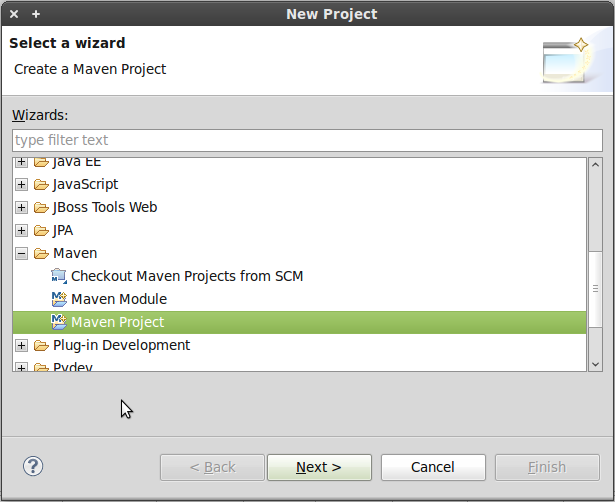
\includegraphics[width=\textwidth]{img/ht01.png}
\caption{Create a new Maven Project.}
\label{fig:maven-project01}
\end{figure}
\begin{figure}
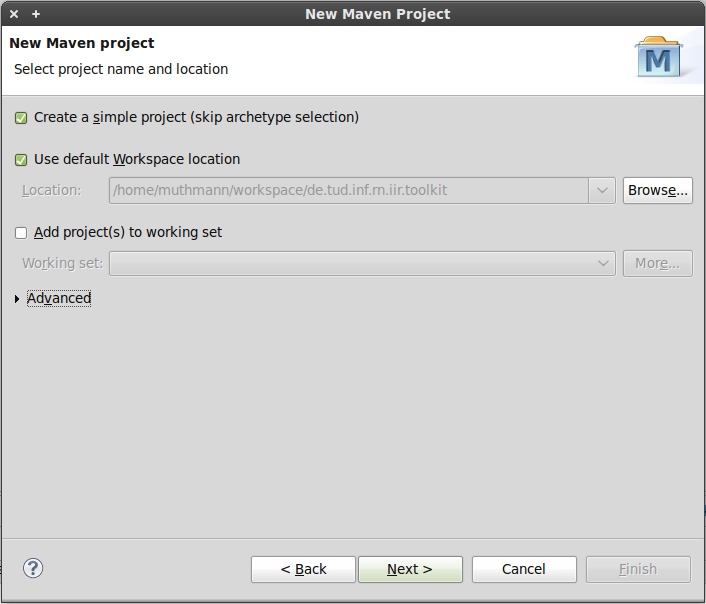
\includegraphics[width=\textwidth]{img/ht02.png}
\caption{Choose to create a simple Maven Project.}
\label{fig:maven-project02}
\end{figure}
\begin{figure}
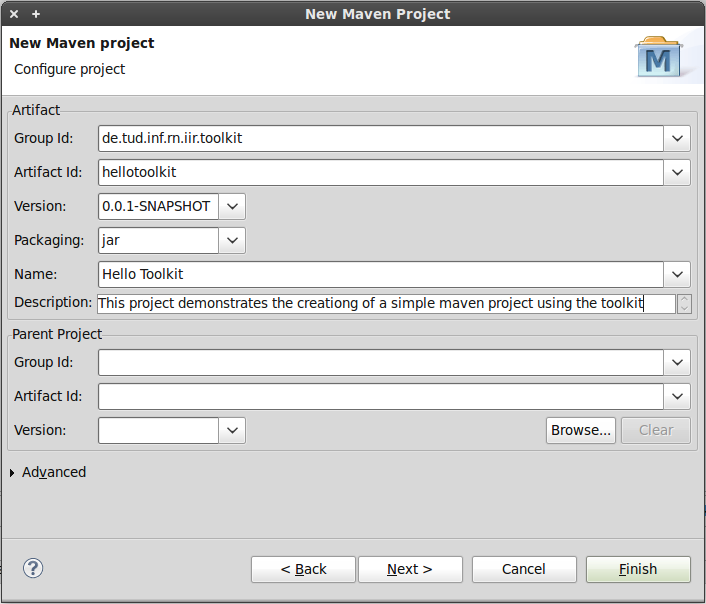
\includegraphics[width=\textwidth]{img/ht03.png}
\caption{Enter detail information about your new Maven Project}
\label{fig:maven-project03}
\end{figure}
\paragraph{Adding the toolkit dependency to the project:} Right click on the new project. In the context menu that appears choose \textit{Maven $\rightarrow$ Add Dependency} (See Fig.~\ref{fig:example-project-context-menu01} and \ref{fig:example-project-context-menu02}).
\begin{figure}
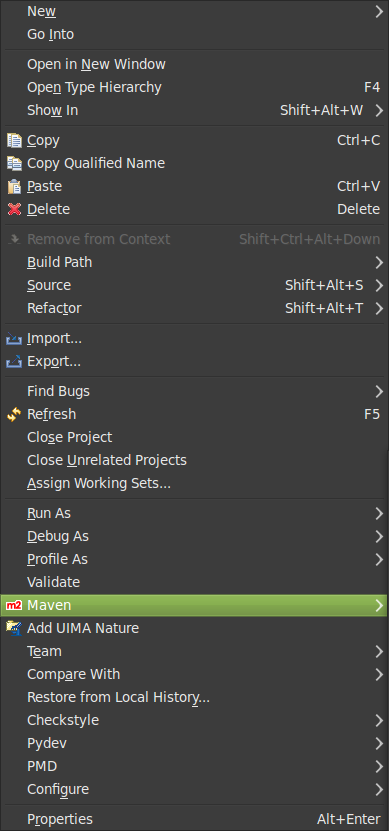
\includegraphics[scale=1]{img/context02.png}
\caption{Maven Project Context Menu. Choose \textit{Maven}}
\label{fig:example-project-context-menu01}
\end{figure}
\begin{figure}
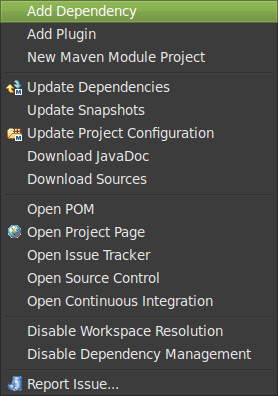
\includegraphics[scale=1]{img/context01.png}
\caption{Create a new Maven project}
\label{fig:example-project-context-menu02}
\end{figure}
A search interface appears (See~\ref{fig:add-dependency01}). If you followed the steps in Section~\ref{sec:buildingthetoolkitusingapachemaven} and installed the toolkit to your local Maven repository, you can type \textit{toolkit} in the search interface (See Fig.~\ref{fig:add-dependency02} and add the dependency with a double click on the \textit{de.tud.inf.rn.iir toolkit} entry. 

Note: If you need to add further dependencies in the future you can use the same steps.
\begin{figure}
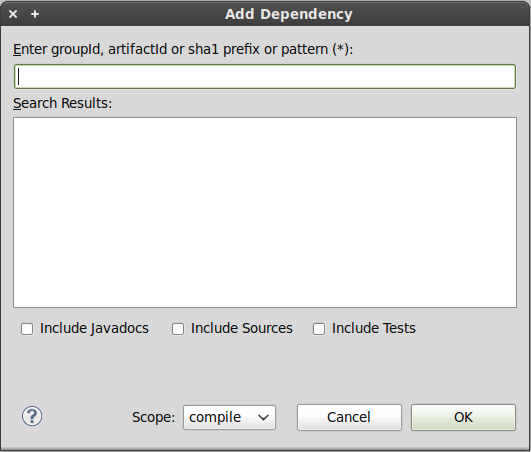
\includegraphics[width=\textwidth]{img/ht04.png}
\caption{Search interface for Maven dependencies.}
\label{fig:add-dependency01}
\end{figure}
\begin{figure}
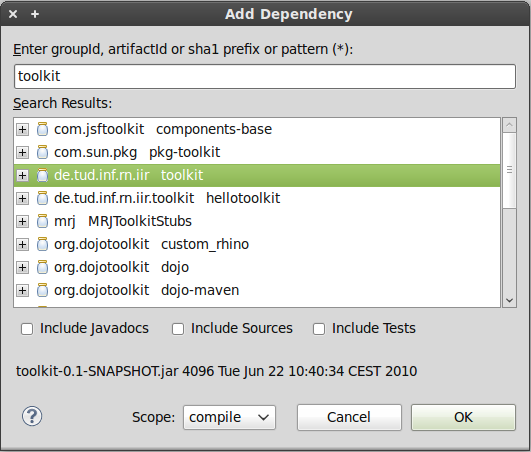
\includegraphics[width=\textwidth]{img/ht05.png}
\caption{Search results for \textit{toolkit}}
\label{fig:add-dependency02}
\end{figure}
The Maven plugin adds the dependency to your pom.xml file, which should look like Fig.~\ref{fig:pom01}.
\begin{figure}
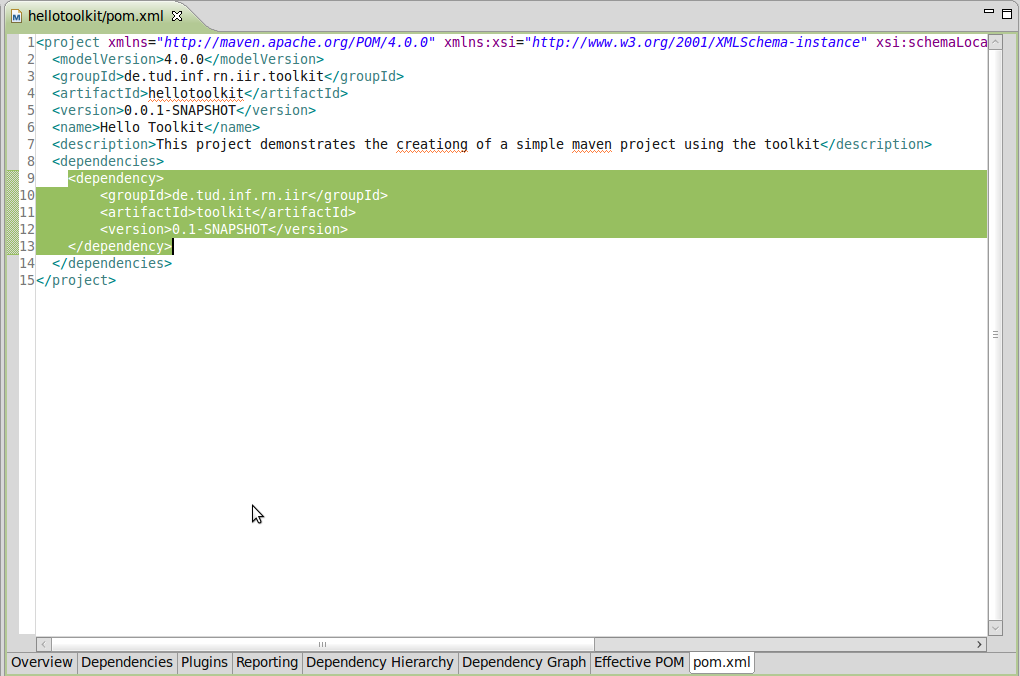
\includegraphics[width=\textwidth]{img/ht06.png}
\caption{POM with added dependency on the TUD IIR Toolkit.}
\label{fig:pom01}
\end{figure}
\paragraph{Configuring your project} Since Maven by default still uses Java 1.4 (very conservative), but the toolkit depends on Java 1.6 (very visionary) you need to configure the Maven Java compiler plugin to use Java 1.6. This is shown in Fig.~\ref{fig:java601}.
\begin{figure}
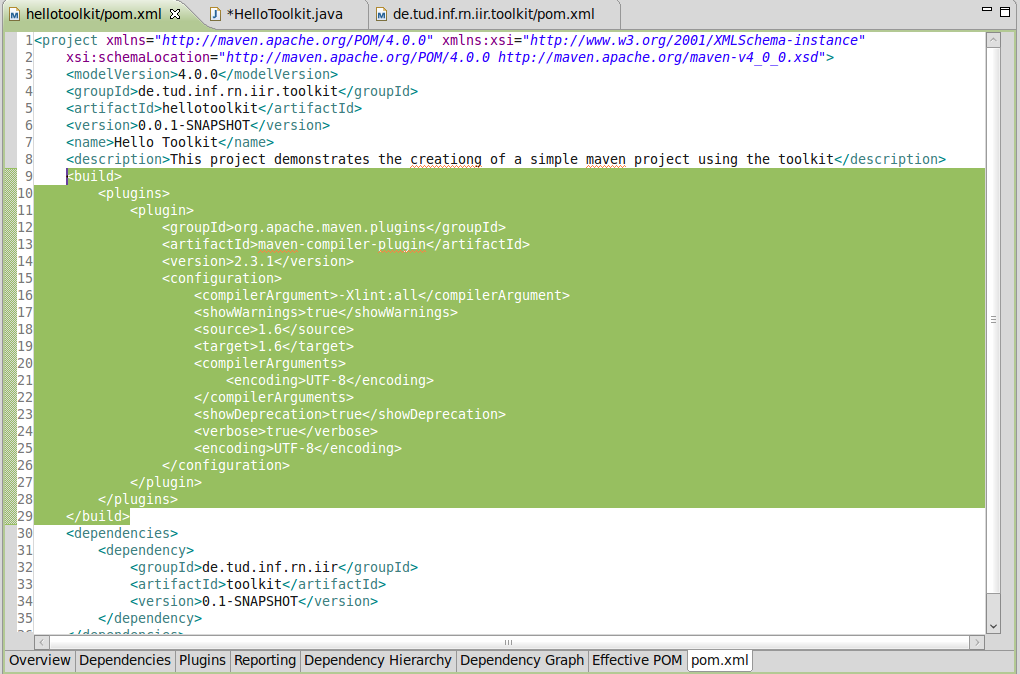
\includegraphics[width=\textwidth]{img/ht07.png}
\caption{Configure the Maven Java compiler to use Java 1.6 instead of 1.4}
\label{fig:java601}
\end{figure}
The same step is necessary to tell Eclipse that it should use Java 1.6 instead of 1.4. For this purpose open the project properties via the context menu for example. In the tree to the left choose \textit{Java Compiler} and change all three entries to 1.6. This is shown in Fig.~\ref{fig:java602} and Fig.~\ref{fig:java603}.
\begin{figure}
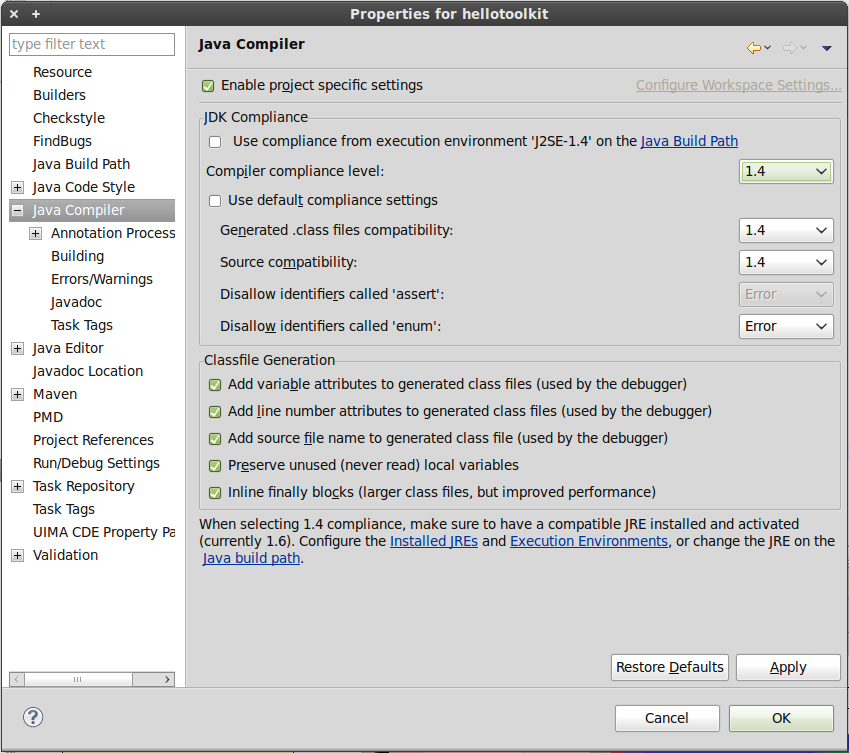
\includegraphics[width=\textwidth]{img/ht08.png}
\caption{Eclipse uses Java 1.4 by default for Maven projects}
\label{fig:java602}
\end{figure}
\begin{figure}
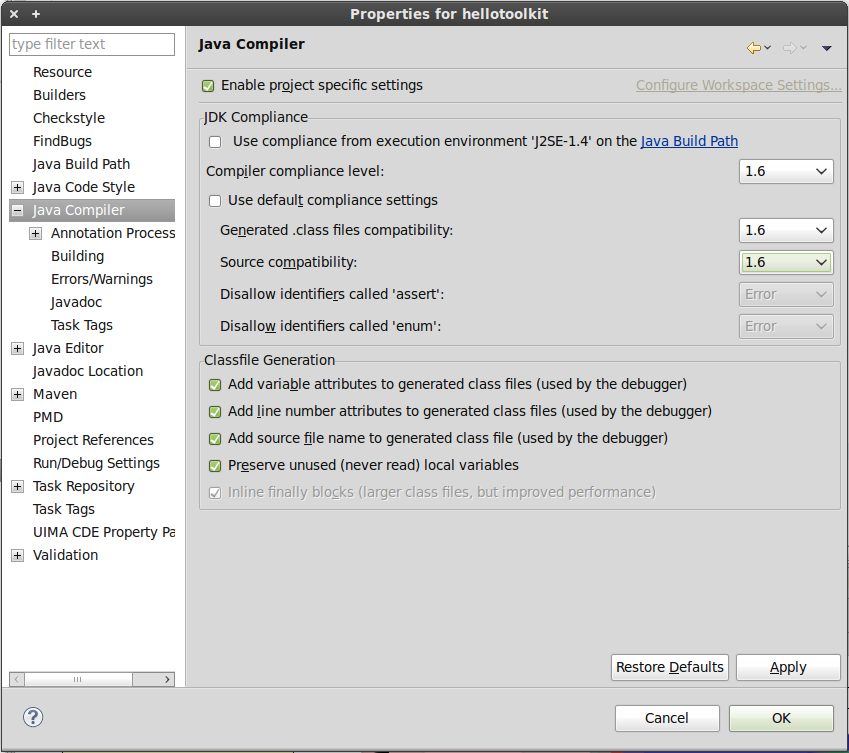
\includegraphics[width=\textwidth]{img/ht09.png}
\caption{configure Eclipse to use Java 1.6}
\label{fig:java603}
\end{figure}
\paragraph{Writing your first toolkit code} Now you can start to write your first code. Your project will already contain the default Maven directory structure. Do not change this structure since Maven depends on it\footnote{Of course you can change Mavens behaviour via the pom.xml but this requires additional configuration not covered by this document. Refer to the Maven documentation under \url{http://maven.apache.org/} for further information.}. As usual we will start with a very simple "Hello World" application. Create a new package \texttt{de.tud.inf.rn.iir.toolkit} and a new class \texttt{HelloToolkit} containing a \texttt{main} method. In this main method you can add actual toolkit code. We used the first example as described in Section~\ref{sec:howto} and search Bing for the term "Hello Toolkit". The example is also shown in Fig.~\ref{fig:hellotoolkit}.
\begin{figure}
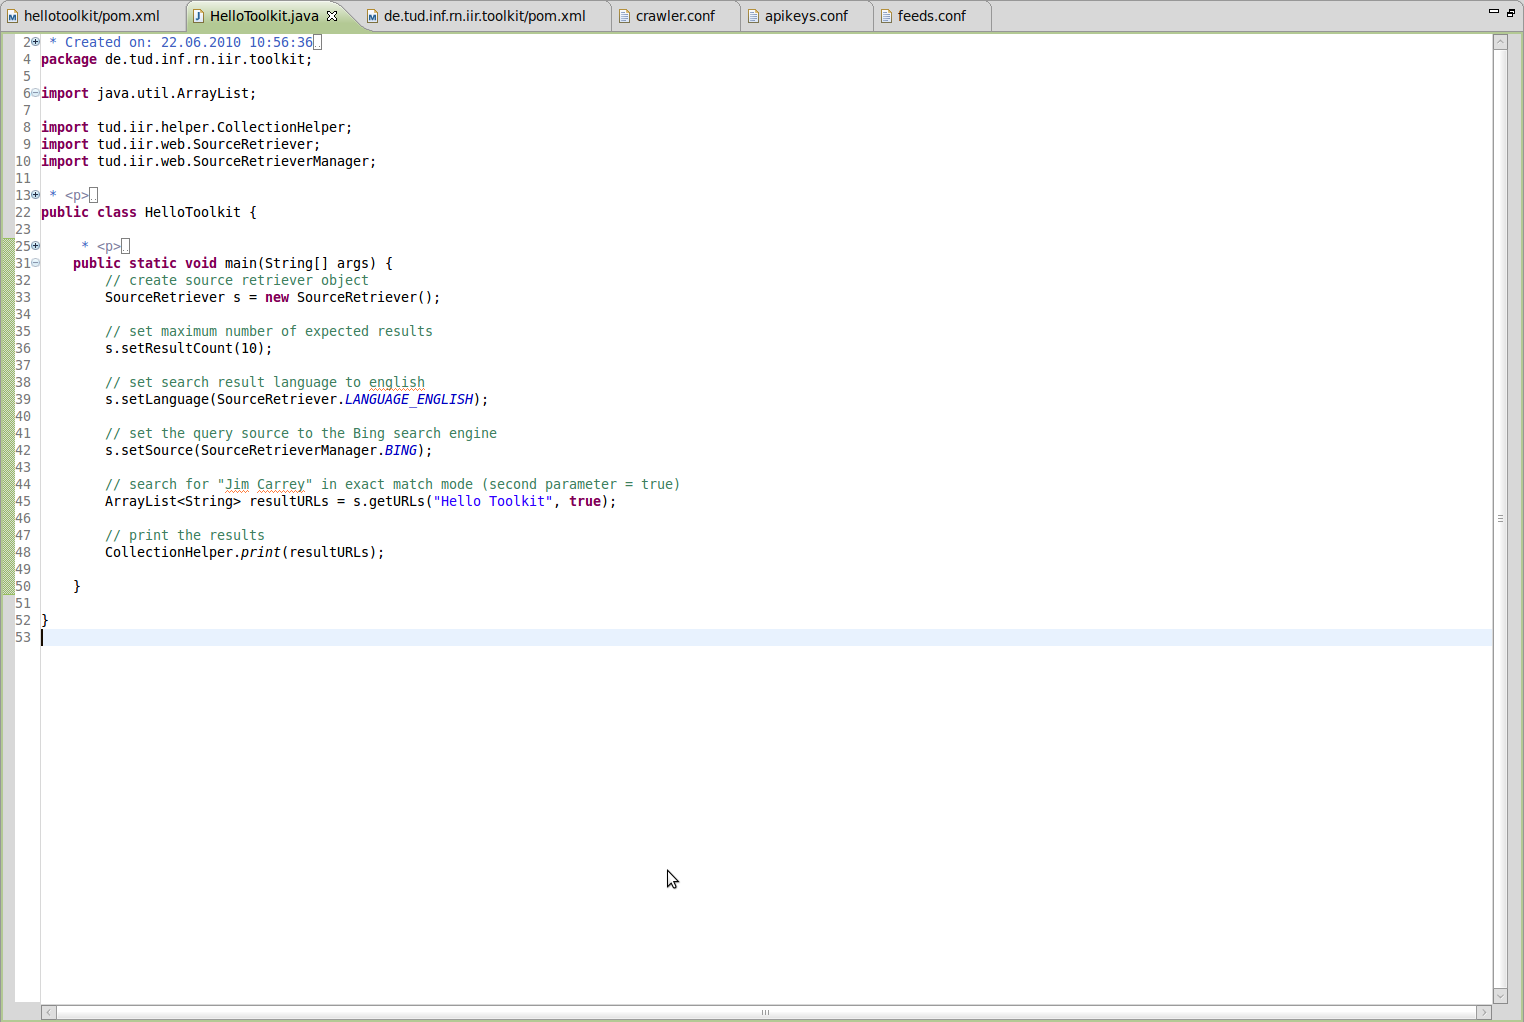
\includegraphics[width=\textwidth]{img/ht10.png}
\caption{"Hello Toolkit" Code}
\label{fig:hellotoolkit}
\end{figure}
For the code to work you need three additional files that are already in the config folder in the toolkit project. These are "crawler.conf", "apikeys.conf" and "feeds.conf". You need to copy them to src/main/resources/config. The folder src/main/resources usually contains all resources that are not Java files but are required by your code. All files are shown in Fig.~\ref{fig:resource01}, \ref{fig:resource02} and \ref{fig:resource03}. Fig.~\ref{fig:structure} shows the final directory and file structure of your project.
\begin{figure}
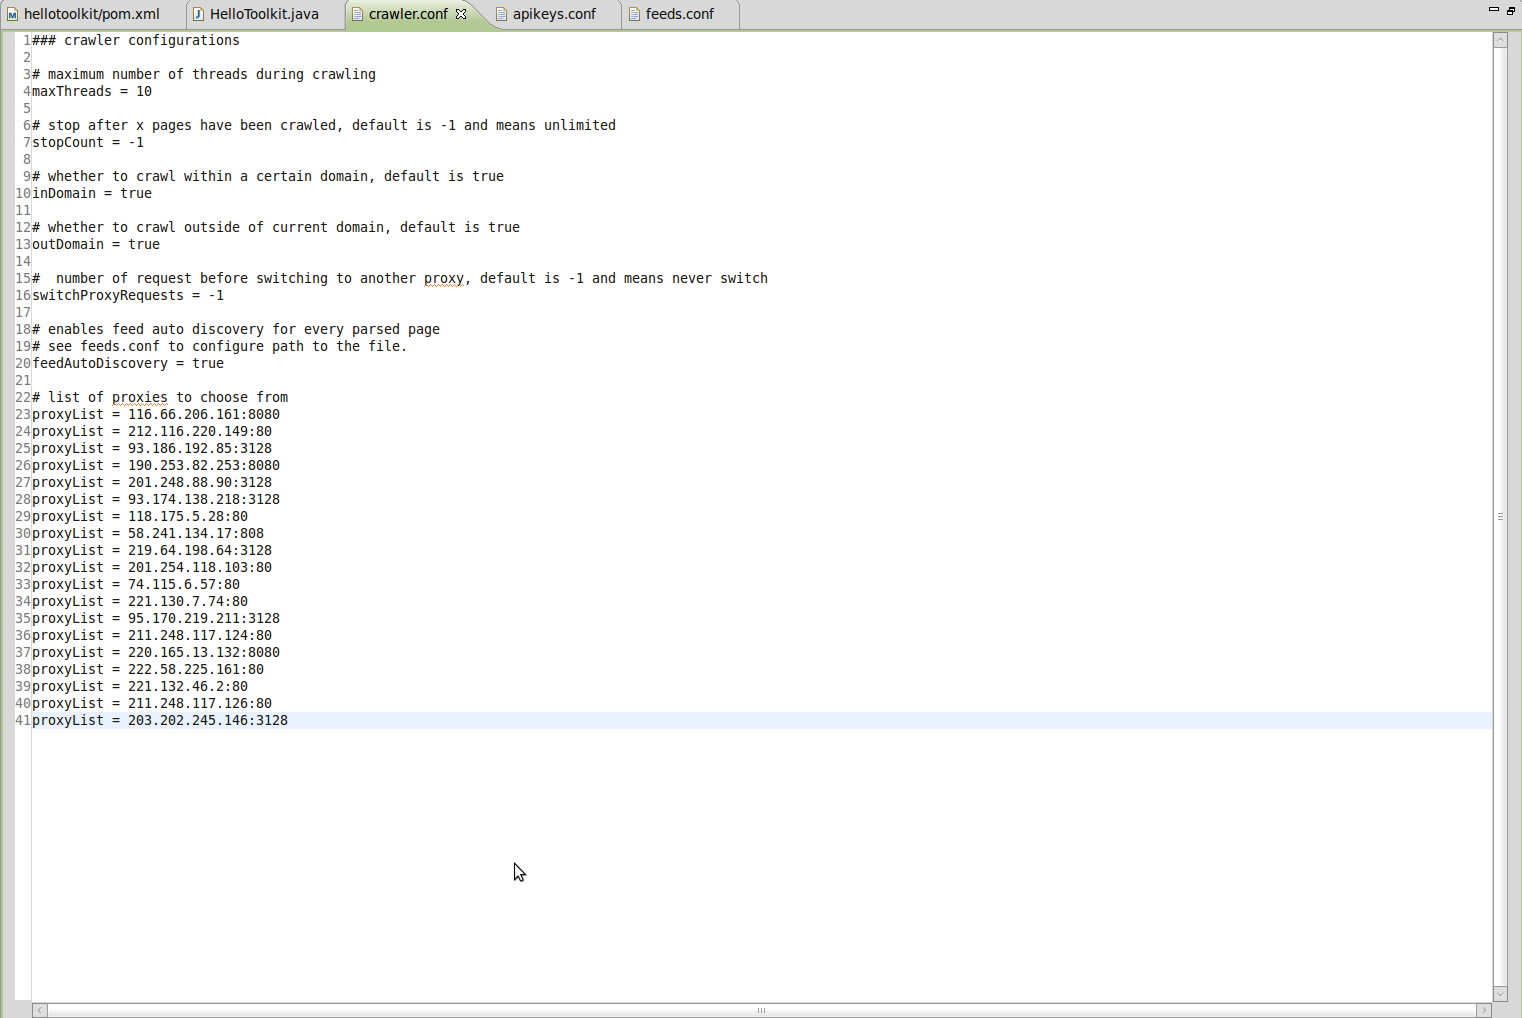
\includegraphics[width=\textwidth]{img/ht11.png}
\caption{Create a new Maven project}
\label{fig:resource01}
\end{figure}
\begin{figure}
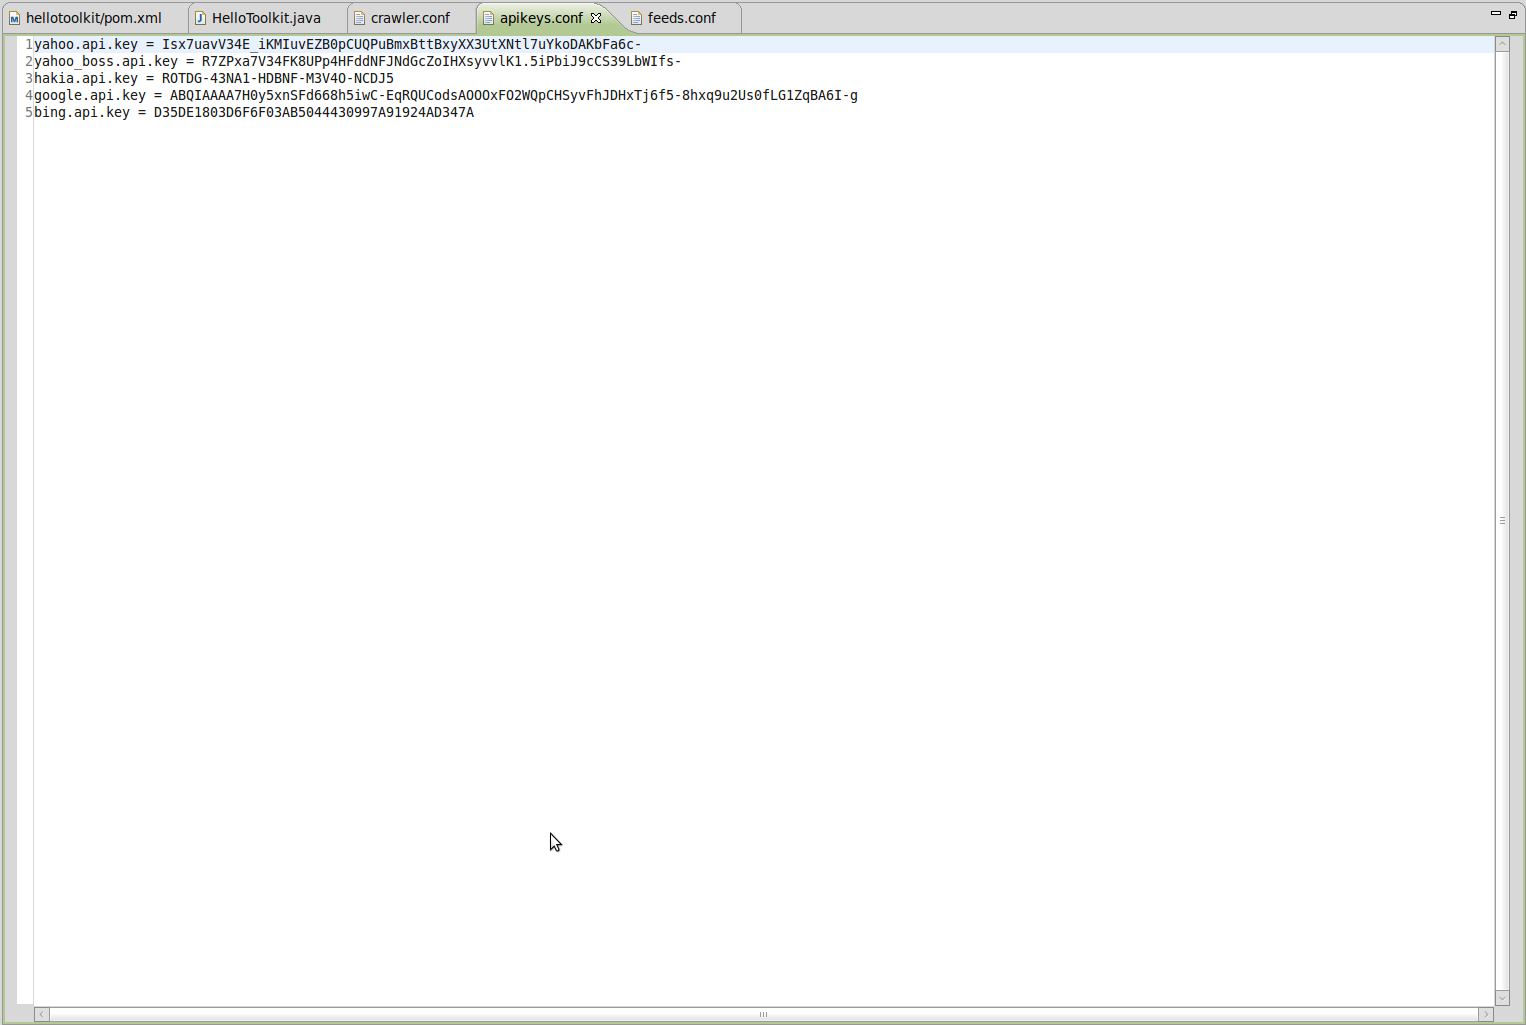
\includegraphics[width=\textwidth]{img/ht12.png}
\caption{Create a new Maven project}
\label{fig:resource02}
\end{figure}
\begin{figure}
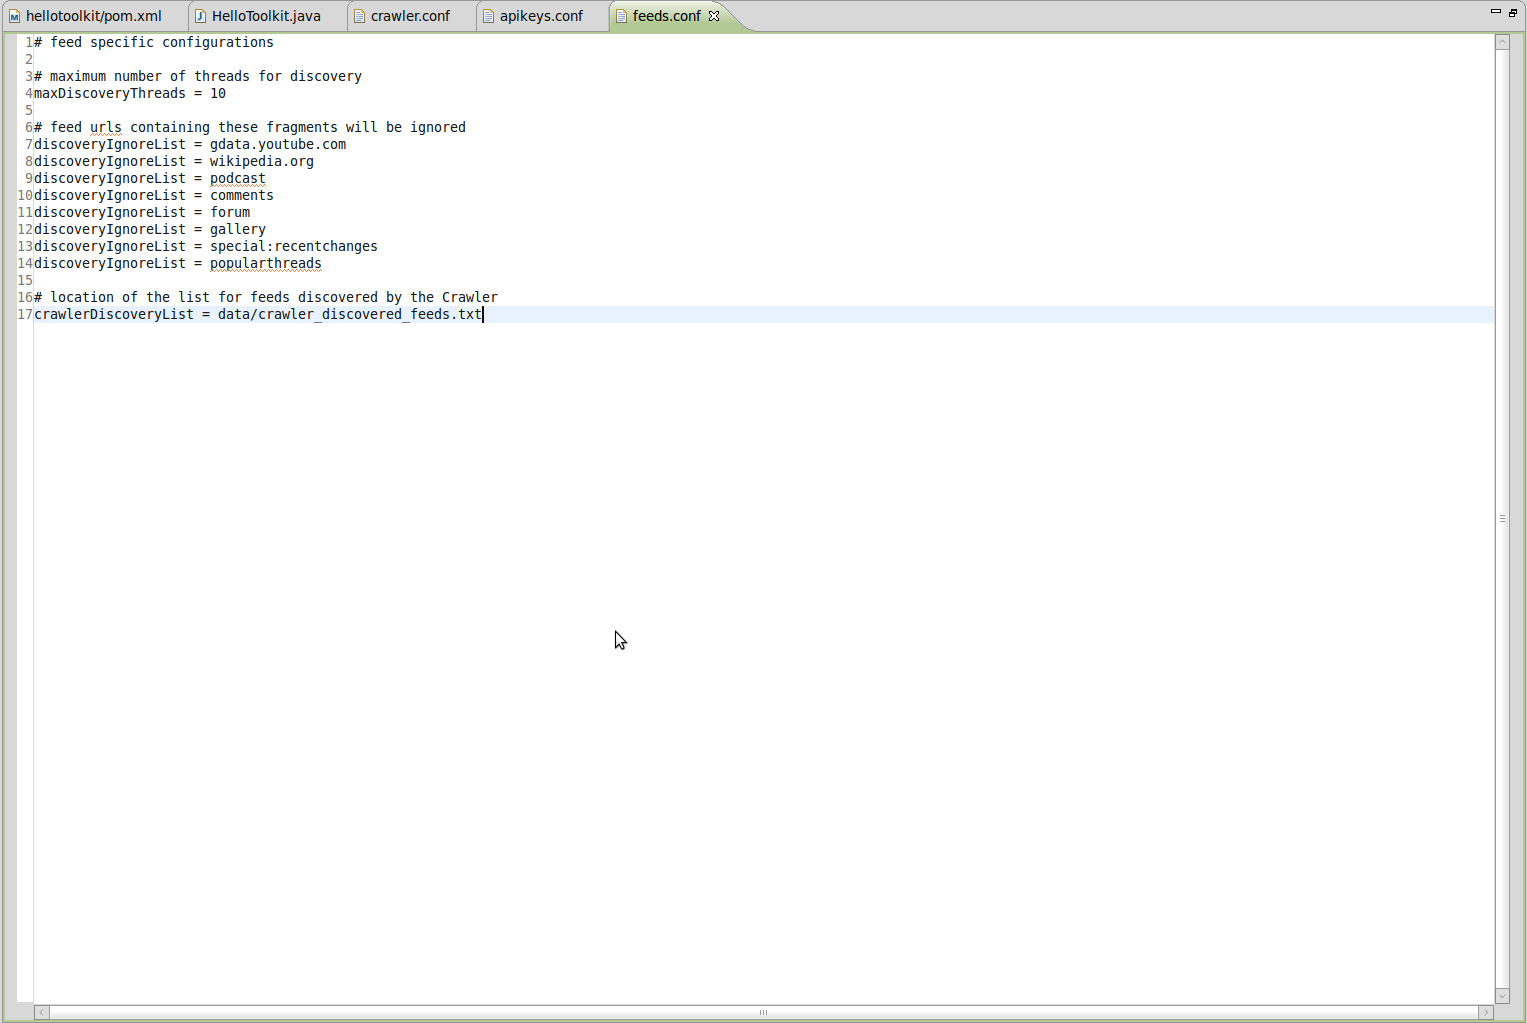
\includegraphics[width=\textwidth]{img/ht13.png}
\caption{Create a new Maven project}
\label{fig:resource03}
\end{figure}
\begin{figure}
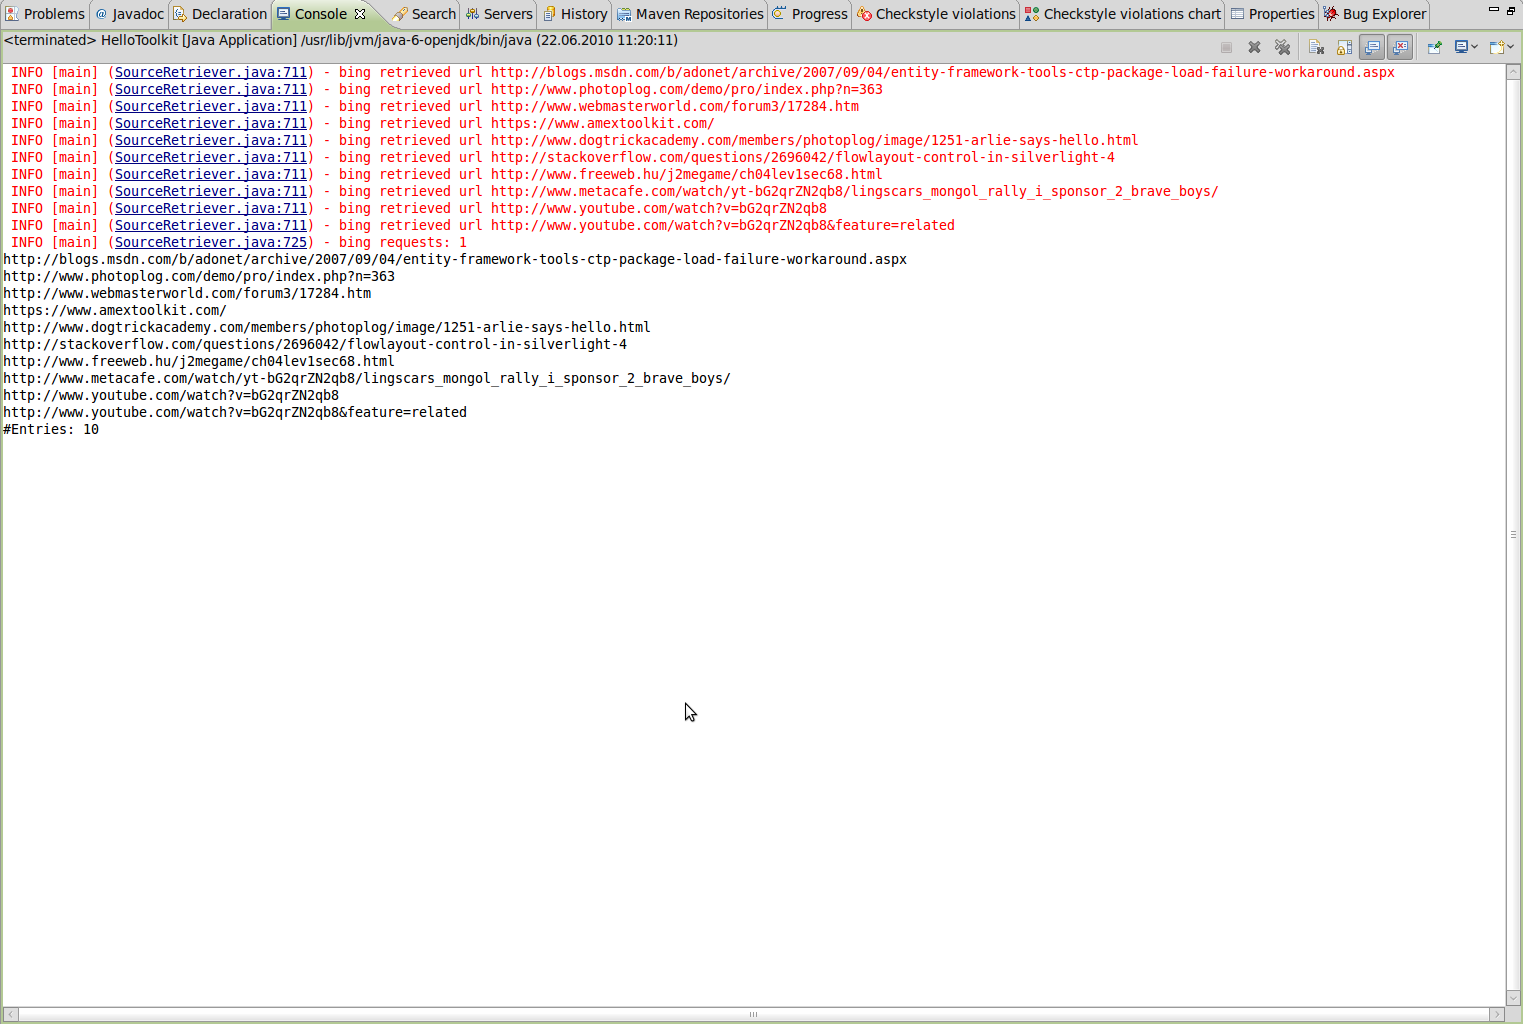
\includegraphics[width=\textwidth]{img/ht14.png}
\caption{Create a new Maven project}
\label{fig:structure}
\end{figure}
With the structure from Fig.~\ref{fig:structure} you can run your project. Just open your projects context menu again, choose \textit{Run As $\rightarrow$ Maven Clean}, then open context menu again choose \textit{Run As $\rightarrow$ Maven Install} and finally choose \textit{Run As $\rightarrow$ Java Application}.

\subsection{Source Retriever}
The source retriever is a module that can query a number of sources such as search engines and web pages with terms and retrieve matching results.
\subsubsection{Basic Features}
Basic features are:
\begin{itemize}
\item Query the Google search engine (unlimited queries, top 64 results only).
\item Query Yahoo search engine (5000 queries per IP and day, top 1000 results).
\item Query Bing search engine (unlimited)
\item Query Hakia search engine.
\item Query Twitter.
\item Query Google Blog search.
\item Query Textrunner web page.
\end{itemize}
Some of the search APIs require API keys which must be specified in the config/apikeys.conf file. See \ref{sec:apikeys.conf} for more information.

\subsubsection{How To}
\label{sec:howto}
The following code snippet shows how to initialize the source retriever and get a list of (English) URLs from the Bing search engine for the exact search ``Jim Carrey''.
\begin{codelisting}
\begin{lstlisting}[frame=tb]
// create source retriever object
SourceRetriever s = new SourceRetriever();
		
// set maximum number of expected results 
s.setResultCount(10);
		
// set search result language to english
s.setLanguage(SourceRetrieve.LANGUAGE_ENGLISH);
		
// set the query source to the Bing search engine 
s.setSource(SourceRetrieverManager.BING);
		
// search for "Jim Carrey" in exact match mode (second parameter = true)
ArrayList<String> resultURLs = s.getURLs("Jim Carrey", true);
		
// print the results
CollectionHelper.print(resultURLs);	
\end{lstlisting}
\end{codelisting}

%\subsection{RankAggregation}

\subsection{Web Crawler}
The web crawler can be used to crawl domains or just retrieve the cleansed HTML document of a single web page.

\subsubsection{Basic Features}
Basic functionalities include:
\begin{itemize}
\item Download and save contents of a web page.
\item Automatically crawl in- and/or outbound links from web pages.
\item Use URL rules for the crawling process.
\item Extract title, description, keywords and body content of a web page.
\item Remove HTML, SCRIPT and CSS tags.
\item Find a sibling page of a given URL.
\item Switch proxies after a certain number of requests to avoid being blocked.
\end{itemize}

\subsubsection{How To}
The following code shows how to instantiate a simple crawler that starts at http://www.dmoz.org and follows all in- and outbound links. The URL of each crawled page is printed to the screen. The crawler will use 10 threads, changes the proxy after every third request and stops after having crawled 1000 pages. Instead of setting the parameters using the code, we can also specify them in the config/crawler.conf file. See \ref{sec:classification.conf} for more information.

\begin{codelisting}
\begin{lstlisting}[frame=tb]
// create the crawler object
Crawler c = new Crawler();

// create a callback that is triggered for every crawled page
CrawlerCallback crawlerCallback = new CrawlerCallback() {
	@Override
	public void crawlerCallback(Document document) {
		// TODO do something with the page
		System.out.println(document.getDocumentURI());
	}
};
c.setCrawlerCallback(crawlerCallback);

// stop after 1000 pages have been crawled (default is unlimited)
c.setStopCount(1000);

// set the maximum number of threads to 10
c.setMaxThreads(10);

// the crawler should automatically use different proxies
// after every 3rd request (default is no proxy switching)
c.setSwitchProxyRequests(3);

// set a list of proxies to choose from
List<String> proxyList = new ArrayList<String>();
proxyList.add("83.244.106.73:8080");
proxyList.add("83.244.106.73:80");
proxyList.add("67.159.31.22:8080");
c.setProxyList(proxyList);

// start the crawling process from a certain page,
// true = follow links within the start domain
// true = follow outgoing links
c.startCrawl("http://www.dmoz.org/", true, true);
\end{lstlisting}
\end{codelisting}

\subsection{FAQ Extractor}
The FAQ extractor can extract question-answer pairs from several structured frequently asked questions pages on websites. The usage is quite simple as shown in the following listing.
\begin{codelisting}
\begin{lstlisting}[frame=tb]
// create a list of question answer pairs
ArrayList<QA> qas = null;

// the URL that contains the FAQ
String url = "http://blog.pandora.com/faq/";

// start extracting question and answers from the URL
qas = QAExtractor.getInstance().extractFAQ(url);

// print the extracted questions and answers
CollectionHelper.print(qas);
\end{lstlisting}
\end{codelisting}

\subsection{Fact Extraction}
The Fact extractor can be used to detect facts in tables on web pages given a URL and optionally a small set of seed attribute names that help the extractor.
\begin{codelisting}
\begin{lstlisting}[frame=tb]
// the URL of the facts
String url = "http://en.wikipedia.org/wiki/Nokia_N95";

// the concept of the attributes
Concept c = new Concept("Mobile Phone");

// a small list of seed attributes
HashSet<Attribute> seedAttributes = new HashSet<Attribute>();
int attributeType = Attribute.VALUE_STRING;
seedAttributes.add(new Attribute("Second camera", attributeType, c));
seedAttributes.add(new Attribute("Memory card", attributeType, c));
seedAttributes.add(new Attribute("Form factor", attributeType, c));

// detect the facts using the seeds from the URL
ArrayList<Fact> detectedFacts = null;
detectedFacts = FactExtractor.extractFacts(url, seedAttributes);
		
// print the extracted facts
CollectionHelper.print(detectedFacts);
\end{lstlisting}
\end{codelisting}

\subsection{Web Page Classification}
The Web Page Classification module can be used to classify web pages by their URL or their full content.

\subsubsection{Basic Features}
The Web Page Classification module has the following basic features:
\begin{itemize}
\item Classify web pages by its URL only.
\item Classify web pages by its full content.
\item Use a combination of URL and full content for classification.
\item Learn, test and reuse models.
\item Simple one-category classification.
\item Hierarchical classification.
\item Multi-category classification (tagging).
\item All algorithms are language independent.
\end{itemize}

\subsubsection{How To}
This section describes how to prepare training and testing data to learn a model and test the classifier.

\paragraph{Preparing the Training/Testing Data}
The data can be specified in a simple text file. There are three classification options, namely, one-category classification, hierarchical classification and multi-category classification. They all require a similar structure of the data.

\subparagraph{One-Category Classification}
We write one URL and one category separated with a single space on each line. For example:
\begin{verbatim}
http://www.google.com search
http://www.fifa.com sport
http://www.oscars.com entertainment
\end{verbatim}

\subparagraph{Hierarchical Classification}
We write one URL and multiple categories separated with a single space on each line. The categories must be in the correct order, so the first category is the main one, all following are subcategories of each other. For example:
\begin{verbatim}
http://www.google.com search search_engine
http://www.fifa.com sport team_sports soccer 
http://www.oscars.com entertainment movies awards usa
\end{verbatim}

\subparagraph{Multi-Category Classification}
We write one URL and multiple categories separated with a single space on each line. The order of the categories (tags) does not matter. For example:
\begin{verbatim}
http://www.google.com search image_search video_search
http://www.fifa.com soccer sport free_time fun ball_game results to_read
http://www.oscars.com entertainment movies films awards watch video stars
\end{verbatim}

\paragraph{Building the Model}
The model is an internal representation of the learned data. After learning a model, a classifier can applied to unseen data. We now have prepared the training and testing data so we can now learn the models. The results of the test will be printed to the console and written to a log file under data/logs. The classifier is saved as a lucene index or a database under the name ``dictionary\_Xclassifier\_Y'' where X is ``url'', ``fullpage'' or ``combined'' and Y is 1 (one-category), 2 (hierarchical) or 3 (multi-category). The model will be written to data/models. How the file is saved can be configured in the config/classification.conf file. See \ref{sec:classification.conf} for more information.

\begin{codelisting}
\begin{lstlisting}[frame=tb]
// create a classifier mananger object
ClassifierManager classifierManager = new ClassifierManager();

// use 80% of the data in the training/testing file as training data
// the rest is used for testing
classifierManager.setTrainingDataPercentage(80);

// specify location of training/testing file
String ttFile = "training_testing_file.txt";

// build and test the model
// the second parameter specifies that we want to use URL features only
// the third parameter specifies that we want to use 
// multi-category classification (tagging)
// the last parameter is set to true in order to train not just test it
classifierManager.trainAndTestClassifier(ttFile,
                                         WebPageClassifier.URL, 
                                         WebPageClassifier.TAG,
                                         true);
\end{lstlisting}
\end{codelisting}

\paragraph{Using the Model}
After we trained a model for a classifier we can apply it to unseen data. Let's use the model we trained for a URL classifier with tagging:

\begin{codelisting}
\begin{lstlisting}[frame=tb]
// create the URL classifier
WebPageClassifier classifier = new URLClassifier();

// create a classification document
ClassificationDocument classifiedDocument = null;

// the web page to be classified
String url = "http://en.wikipedia.org/wiki/Computer";

// use the classifier to classify a web page to multiple categories
// using URL features only
classifiedDocument = classifier.classify(url, WebPageClassifier.TAG);

// print out classification results
System.out.println(classifiedDocument);
\end{lstlisting}
\end{codelisting}

\subsection{Helpers}
The toolkit contains many helper functionalities for reoccurring tasks in the tud.iir.helper package.
The following code snippet shows several sample usages of some of the functions.

\begin{codelisting}
\begin{lstlisting}[frame=tb]
// sort a map by its value in ascending order (2nd parameter = true)
Map m = CollectionHelper.sortByValue(map, true);

// reverse a list
List l = CollectionHelper.reverse(list);

// print the contents of a collection
CollectionHelper.print(collection);

// get the runtime of an algorithm and print it (2nd parameter = true)
long startTime = System.currentTimeMillis();
for (int i = 0; i < 10000; i++) {
	int c = i * 2;
}
DateHelper.getRuntime(t1, true);

// (de) serialization of objects
FileHelper.serialize(obj, "obj.ser");
Object obj = FileHelper.deserialize("obj.ser");

// rename, copy, move and delete files
FileHelper.rename(new File("a.txt"), "b.txt");
FileHelper.copyFile("src.txt", "dest.txt");
FileHelper.move(new File("src.txt"), "dest.txt");
FileHelper.delete("src.txt");

// get files from a folder
File[] files = FileHelper.getFiles("folder");

// zip and unzip a text
FileHelper.zip("text", "zipFile.zip");
String t = FileHelper.unzipFileToString("zipFile.zip");

// perform some action on every line of an ASCII file
final Object[] obj = new Object[1];
obj[0] = 1;

LineAction la = new LineAction(obj) {
  
    @Override
    public void performAction(String line, int lineNumber) {
        System.out.println(lineNumber + ": " + line + " " + obj[0]); 
    }
}
FileHelper.performActionOnEveryLine(filePath, la);

// round a number with a number of digits
double r = MathHelper.round(2.3333, 2);

// calculate n-grams of a string
Set<String> nGrams = StringHelper.calculateNGrams("abcde", 3);

// English singular word to plural
String p = StringHelper.wordToPlural("city");

// remove HTML tags
String r = StringHelper.removeHTMLTags("<a>abc</a>",
                                       true, true
                                       true, true);

// trim a string
String t = StringHelper.trim(" _to trim++++");

// get singular or plural of an English word
String plural = StringHelper.wordToPlural("city");
String singular = StringHelper.wordToSingular("cities");

// reverse a string
String r = StringHelper.reverse("abc");

// encode and decode base64
String e = StringHelper.encodeBase64("abc");
String d = StringHelper.decodeBase64(e);

\end{lstlisting}
\end{codelisting}

\section{Reference Libraries}
The TUDIIR Toolkit makes excessive use of third party libraries. We do not intend to re-implement code but rather to built on it and create something superior. Here an incomplete list of libraries the toolkit uses:
\begin{itemize}
\item Alchemy API \cite{alchemy} to query the services of Alchemy.com.
\item Apache Commons \cite{apachecommons} for many standard tasks in string and number manipulation and more.
\item Fathom \cite{fathom} to measure readability of English text.
\item iText \cite{itext} for creating PDF documents.
\item Jena \cite{jena} for reading and writing ontology files.
\item jFreeChart \cite{jfreechart} for creating charts.
\item jYaml \cite{jyaml} to read and write YAML files.
\item Log4j \cite{log4j} for logging.
\item Lucene \cite{lucene} for indexing and making learned models persistent.
\item NekoHTML \cite{nekohtml} to clean up the HTML of web pages in order to process them correctly.
\item SimMetrics \cite{simmetrics} to calculate similarities of strings.
\item Twitter4j \cite{twitter4j} to query the Twitter API.
\item Weka \cite{weka} for machine learning.
\end{itemize}

\section{History}
The foundation of the toolkit code came out of the WebKnox project\cite{webknox} that was started in 2008.% Now, components of the Aletheia project\footnote{\url{http://www.aletheia-projekt.de}} and the Effingo project\footnote{\url{http://www.effingo.de}}

The code is in development by students of the Dresden University of Technology. Contributors are:
\begin{itemize}
\item Christopher Friedrich
\item Martin Gregor
\item Philipp Katz
\item David Urbansky
\item Robert Willner
\item Martin Werner
\end{itemize}

\begin{thebibliography}{99}
%\bibitem{amari} S-I. Amari. {\bf Differential Geometrical Methods in
%Statistics}, Springer Lecture Notes in Statistics 28,
%Springer-Verlag, Berlin 1985.
%\end{thebibliography}
\bibitem{apachecommons} \url{http://commons.apache.org/}
\bibitem{itext} \url{http://itextpdf.com/}
\bibitem{jena} \url{http://jena.sourceforge.net/}
\bibitem{jfreechart} \url{http://www.jfree.org/jfreechart/}
\bibitem{log4j} \url{http://logging.apache.org/log4j/}
\bibitem{lucene} \url{http://lucene.apache.org/}
\bibitem{nekohtml} \url{http://nekohtml.sourceforge.net/}
\bibitem{simmetrics} \url{http://www.dcs.shef.ac.uk/~sam/simmetrics.html}
\bibitem{fathom} \url{http://www.representqueens.com/fathom/}
\bibitem{twitter4j} \url{http://twitter4j.org/en/index.html}
\bibitem{alchemy} \url{http://www.alchemyapi.com/tools/}
\bibitem{jyaml} \url{http://jyaml.sourceforge.net/}
\bibitem{weka} \url{http://www.cs.waikato.ac.nz/ml/weka/}
\bibitem{webknox} \url{http://www.webknox.com}
\bibitem{codingStandards} \url{http://net.tutsplus.com/tutorials/html-css-techniques/top-15-best-practices-for-writing-super-readable-code/}
\end{thebibliography}
\end{document}
